Жизненный цикл процесса начинается с того, что его кто-то порождает. Единственный процесс, который никто не порождает, это процесс init. Порождение процесса осуществляется с помощью fork (2) или vfork (2). 

Первая стадия в жизни процесса --- \textbf{“инициализация“}. В это время ядро производит подготовительные работы к дальнейшей работе процесса. На самом деле, это не совсем состояние, но логически для пользователя оно существует.

\begin{figure}[htbp]
  \centering
  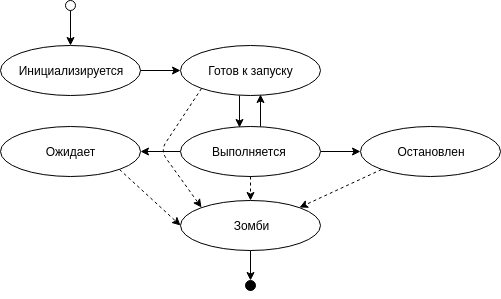
\includegraphics[width=0.7\textwidth]{./processes-and-threads/processes/lifecycle/proc-lifecycle.png}
\end{figure}

Когда инициализация процесса завершается --- он оказывается в стадии \textbf{“готов“}. С этого момента процесс находится в ожидании момента, когда его выберет планировщик процессов и даст ему какой-то квант процессорного времени.

При получении процессорного времени процесс переходит в состояние \textbf{“выполняется“}. Выполняться процесс может в режиме ядра --- при осуществлении системных вызовов, прерываний и в режиме задачи --- выполнять инструкции процессора. По окончании квоты времени, процесс может снова вернуться в состояние \textbf{“готов“}.

Также из состояния “выполняется“ процесс может перейти еще в два состояния --- \textbf{“остановлен“} и \textbf{“ожидает“}. Если он остановлен, то он остановлен пользователем (например, получен сигнал SIGSTOP). Ожидание наступает тогда, когда процессу нужны какие-то ресурсы. Как только условие, которого ждет процессор, выполняется, он переходит в состояние \textbf{“готов“}, то есть ожидает своей очереди на выполнение. 

Из каждого состояния процесс может перейти в в состояние \textbf{“зомби“}. Этот процесс нужен для того, чтобы родительский процесс мог получить код возврата этого процесса. Это промежуточное состояние --- процесса уже нет, но он технически еще есть. Тем не менее, это самое что ни на есть валидное состояние. 

\textbf{В какой момент процесс окончательно исчезает из таблицы процессов?}

После того как его родительский процесс вызовет wait (2), waitpid (2), waitid(2) - позволяет завершить процесс, если он таки стал зомби. 

Традиционная проблема --- порождая процесс, необходимо в какой-то момент сказать ему wait (2), чтобы не плодить зомби. В противном случае у вас может закончится лимит на создание новых процессов. 

\textbf{Что происходит с зомби, если его родитель не вызвал wait (2), а погиб?}

Его родителем становится init. Для всех процессов, которые становятся его потомками он делает wait (2). По факту, если вы написали какой-то код, который выполняет некоторое количество процессов после чего завершился, то на самом деле зомби в системе не останутся, т.к. после того как ваш основной процесс завершился, то потомков этого процесса подхватит init и он сам вызовет для них wait (2).